\chapter{Results}
\section{Important Quantities from Our Model}
As shown in the previous chapter, our model describes the change in allele frequencies over time and space. Evolutionary forces act to shape the distribution of alleles across our simulated geographic habitat. There are two immediate questions that we will utilize our model to answer:

\begin{enumerate}
    \item How much of the allele do we expect to observe?
    \item Where can we expect to find the allele?
\end{enumerate}


For a more intuitive understanding of what each of these questions represent, let us examine the raw simulation output from our model. We simulate a single genetic locus and record the frequency of the minor, or \textit{focal} allele $f(a)$ after thousands of simulated generations. Allele frequencies vary across geographic position, but tend to be higher in some neighboring demes. This represents the localization of rare alleles observed in natural populations. \cite{1000_genomes} \cite{geerlings_2018} \cite{novembre_marcus_2017} 


\begin{figure}[h]
    \centering
    \textbf{Allele frequency heatmap in 2D simulation} \par \medskip
    \hspace*{+1.5cm}  
    \includegraphics[scale=1]{img/heatmap.png}
    \caption{The geographic distribution of allele frequencies in a single simulation with a single set of evolutionary parameters ($\mu,s,m,N$). We allow for thousands of generations of time to pass to allow our simulation to approach equilibrium. Alleles exist in clusters throughout the spatial environment.}
    \label{fig:geog_sim}
\end{figure}


We observe that demes with the highest focal allele frequencies tend to exist in clusters (Figure: \ref{fig:geog_sim}). The size of these clusters illustrate the geographic range of the allele. New alleles come into existence at one particular location. Some of these will reach higher frequencies in the population and some will spread farther beyond their initial position. The average frequency in these clusters tells us how much of the allele we can expect to observe, and the size of the clusters tells us where we can expect to observe it. It is clear that alleles that reach, on average, higher frequencies will be easier to observe. We will calculate the average allele frequency and the geographic range of an allele analytically and confirm our predictions with simulation data.


\subsection{The average allele frequency}
Recall that we simulate changes in allele frequency according to the equation:

\begin{equation}
    \tag{\ref{eq:model} revisited}
    df_r=[\mu(1-2f_r)-sf_r (1-f_r ) + m (f_{r-1}+f_{r+1}-2f_r)]dt+\sqrt{\frac{f_r (1-f_r )}{N}} dB_{t,r}
\end{equation}

We want to solve this equation for the average, or expected, allele frequency at equilibrium $\frac{df}{dt} = 0$. We take the expectation over $t$ and $r$. Using the Law of Total Expectation, we can show:

\begin{equation}
    \begin{split}
        0 &= E[\mu(1-2f_r)-sf_r (1-f_r ) + m (f_{r-1}+f_{r+1}-2f_r)+\sqrt{\frac{f_r (1-f_r )}{N}} dB_{t,r}] \\ 
        & \text{Using equation \ref{eq:exp_ss}:} \\
        &= E[\mu(1-2f_r)-sf_r (1-f_r )] + 0 + E[\sqrt{\frac{f_r (1-f_r )}{N}} dB_{t,r}]  \\
        & \text{Using $E[dB_{t,r}] = 0$ (drift property):} \\
        &= E[\mu(1-2f_r)-sf_r (1-f_r )] + 0  \\
        &= E[\mu(1-2f_r)] - E[sf_r (1-f_r)] \\
        &= \mu - 2\mu E[f] - sE[f] + sE[f^2] \\
        E[f](2\mu + s) &= \mu + sE[f^2] \\
        E[f] &= \frac{\mu + sE[f^2]}{2\mu + s} \\
        & \text{Using $sE[f^2] << \mu$ (rare allele assumption):} \\
        E[f] &\approx  \frac{\mu}{2\mu + s}  \\
        & \text{Using $2\mu << s$: (strong selection assumption)} \\
        \therefore E[f] &\approx \frac{\mu}{s} 
    \end{split}
\end{equation}


Thus, even with geographic population structure, our model accords with the well-known \textit{mutation-selection balance} result \cite{fisher_1930} in well-mixed populations. The average allele frequency can be approximated as the ratio of the mutation rate to the selection coefficient. As we increase the selection coefficient, selection removes the allele from the population at a faster rate. This implies that the allele will be rarer on average. note that this result is independent of population size and migration. We validate this relationship with simulations:

\begin{figure}[h]
    \centering
    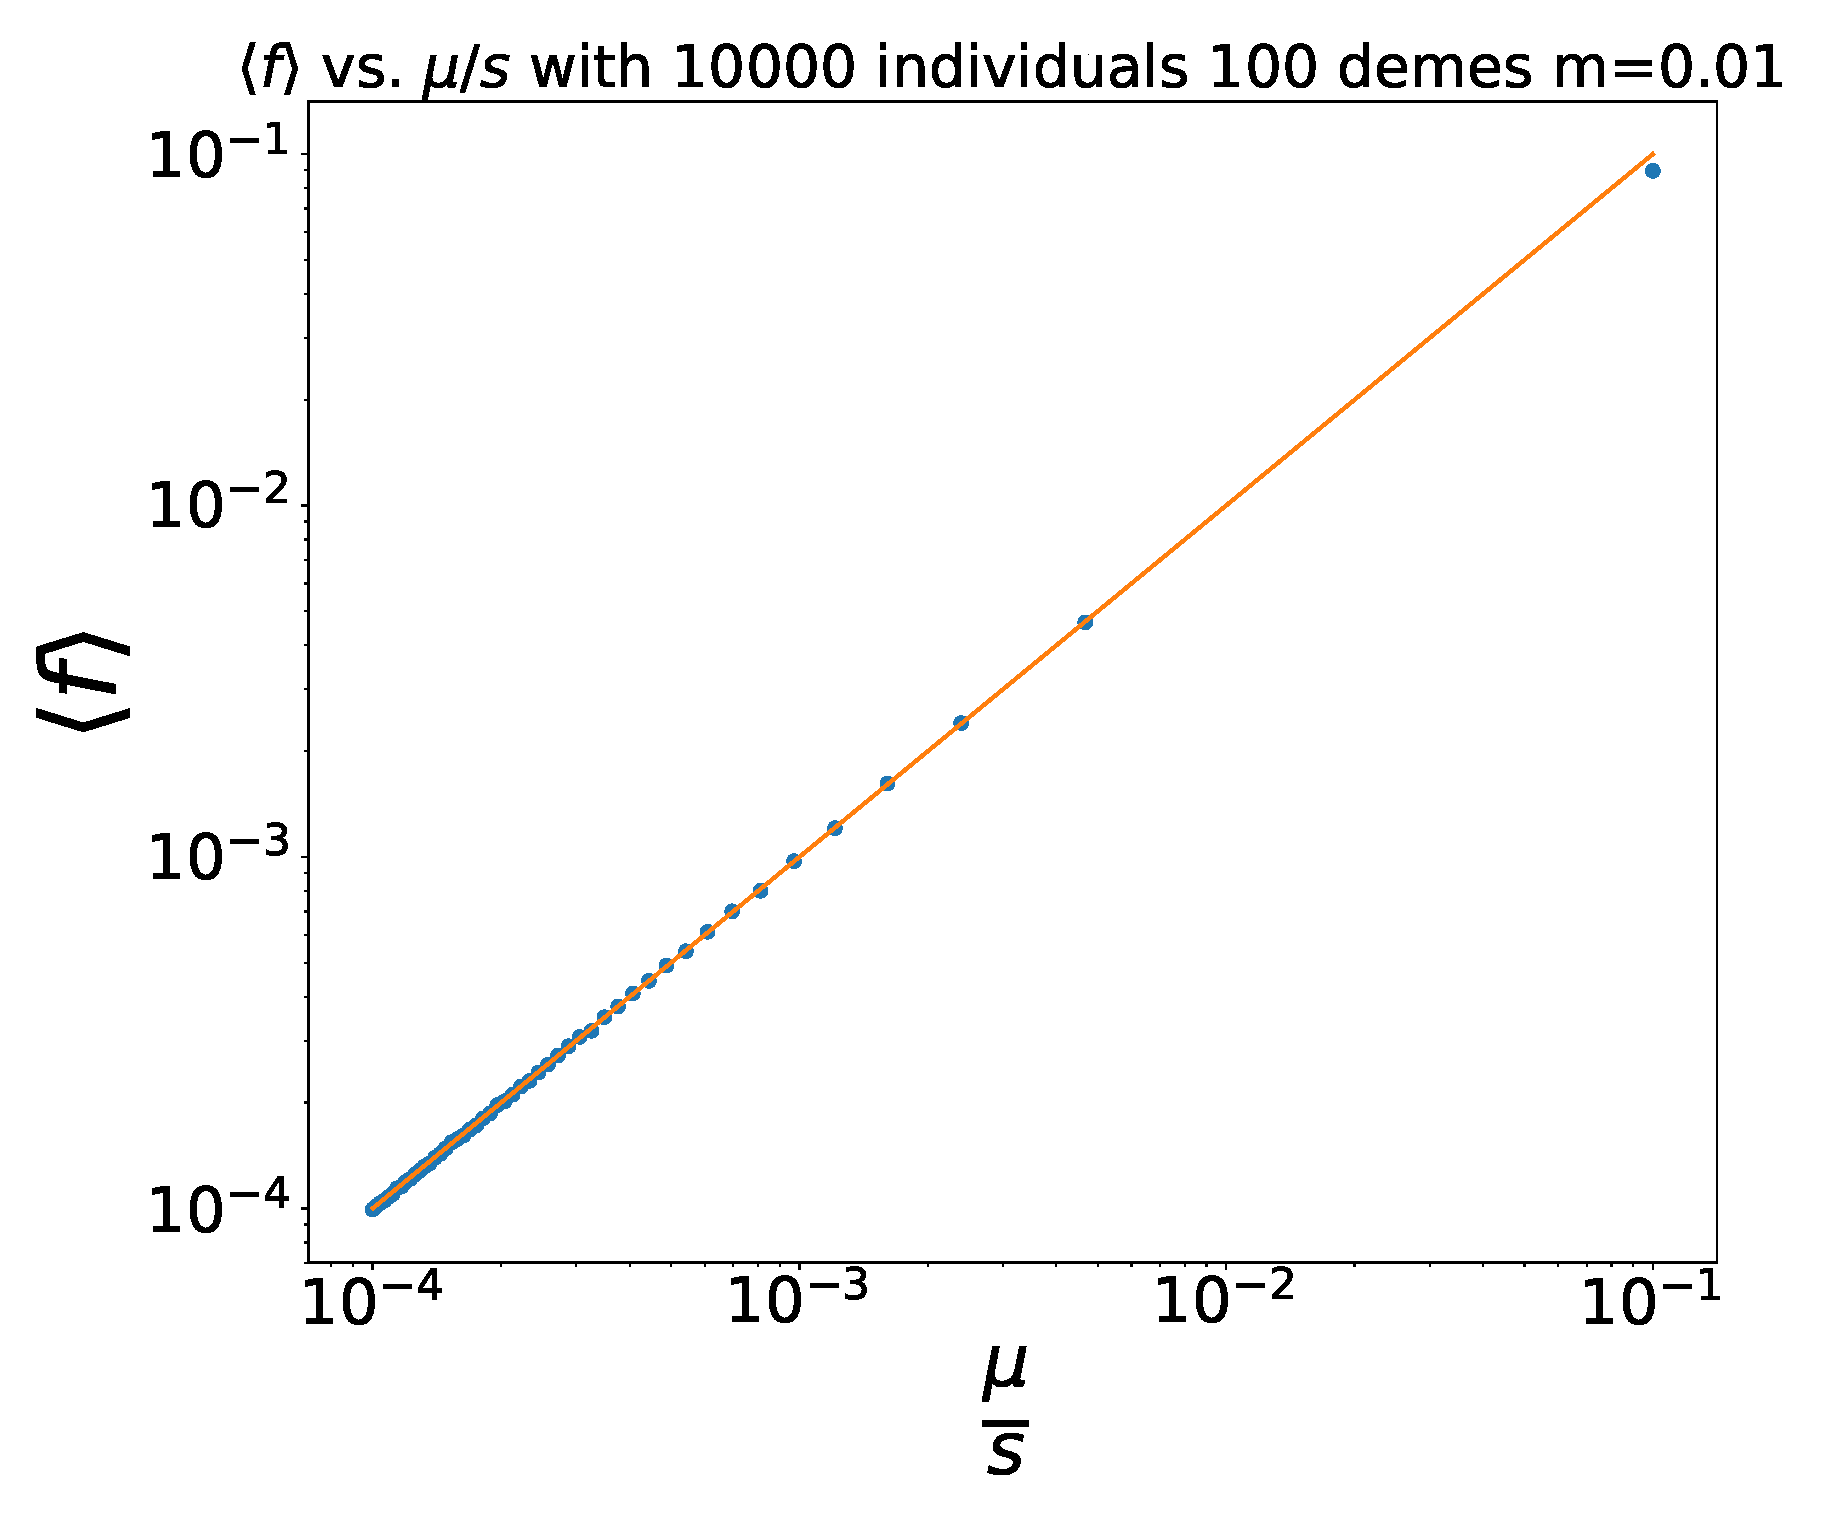
\includegraphics[scale=0.4]{img/fig1.eps}
    \caption{The average allele frequency $E[f] = \langle f \rangle$ is proportional to the ratio $\frac{\mu}{s}$. Each point shows the computed mean frequency value from a simulation run to equilibrium and the mutation-selection ratio used. The line shown has slope $1$ and intercept $0$. }
    \label{fig:avg_freq}
\end{figure}

$\frac{\mu}{s}$ tells us, on average, how much of the allele we expect to observe at any location. The mutation rate in mammalian genomes is approximately constant across genes (order $10^{-9}$ per base pair per year). \cite{kumar_subramanian_2002} \cite{scally_2016} Therefore, the main force driving average allele frequencies is selection. This result validates our previous intuition that large-effect/largely deleterious alleles tend to be rare.

\newpage
\subsection{The geographic range of the allele}
In this section we examine the forces driving the geographic range of the allele. We expect rare alleles to be more geographically isolated, and we have just shown that selection determines allele rarity. Therefore, we are particularly interested in how changing rates of selection and migration influences the geographic patterns of allele frequencies. 


Let us examine the parameters $m$ and $s$ in relation to one another. Both parameters are of dimensions $[m] = [s] = [time^{-1}]$. Therefore, their reciprocals are of dimensions $[time]$. The value $\frac{1}{m}$ is essentially the time an allele takes to migrate between demes. Another way to interpret this is that \textit{increasing} $m$ \textit{decreases} the time an allele spends in the same deme. Likewise, the value $\frac{1}{s}$ is essentially the time before an allele is removed by selection, i.e. the \textit{lifespan} of the allele. We examine the three possible relationships:

\noindent\begin{tabularx}{\textwidth}{@{}XXX@{}}
  \begin{equation} 
           \frac{1}{s} < \frac{1}{m}
    \implies \frac{m}{s} < 1 
    \label{eq:ms_less_1}
  \end{equation} &
  \begin{equation}
           \frac{1}{s} = \frac{1}{m}
    \implies \frac{m}{s} = 1 
    \label{eq:ms_equal_1}
  \end{equation} &
  \begin{equation}
           \frac{1}{s} > \frac{1}{m}
    \implies \frac{m}{s} > 1 
    \label{eq:ms_greater_1}
  \end{equation}
\end{tabularx}

Inequality \ref{eq:ms_less_1} states that the lifespan of an allele is shorter than the time it takes the allele to move to another deme. In this scenario, we expect changes in the allele frequency at one deme to not strongly affect the allele frequency in nearby demes. Changes in allele frequencies in nearby demes should be mostly \textit{uncorrelated}. If \ref{eq:ms_equal_1} is true, then neither force has an advantage over the other and we expect to see some correlation of allele frequencies in nearby demes. Some alleles have time to migrate to nearby demes before they are removed by selection. The final case of inequality \ref{eq:ms_greater_1} predicts that alleles have lifespans longer than the time it takes them to migrate. Therefore, we expect to see strong correlation in allele frequencies of nearby demes. We simulate frequency trajectories in a two-deme model under each of the three possible $\frac{m}{s}$ relationships.


\begin{figure}[h]
    \centering
    \hspace*{-2cm}
    \includegraphics[scale=0.5]{img/low_high_migration.JPG}
    \caption{As }
    \label{fig:}
\end{figure}

\begin{figure}[h]
    \centering
    \includegraphics[scale=0.3]{img/correlation_curve.JPG}
    \caption{}
    \label{fig:}
\end{figure}




\section{Computing the Expected Site Frequency Spectrum}

\begin{figure}[h]
    \centering
    \includegraphics[scale=0.3]{img/sampling_curves.png}
    \caption{}
    \label{fig:}
\end{figure}

\begin{figure}[h]
    \centering
    \includegraphics[scale=0.3]{img/fig4.eps}
    \caption{sfs}
    \label{fig:}
\end{figure}


\section{Measuring Missing Heritability}

\begin{figure}[h]
    \centering
    \includegraphics[scale=0.3]{img/sampling_heatmap.JPG}
    \caption{}
    \label{fig:}
\end{figure}


\begin{figure}[h]
    \centering
    \includegraphics[scale=0.3]{img/H_plot_s_0.0001_m_0.1_pop_size_1e-5.png}
    \caption{}
    \label{fig:}
\end{figure}




%%%%% extra
